\chapter{Mohr-Coulomb model}

\section{Introduction}
The classical Mohr-Coulomb model is a workhorse of rock and soil plasticity modeling.
This model is typically hard to implement for implicit codes because of the
difficulties encountered in computing tangent stiffness matrices near the corners (as viewed from the
hydrostatic axis).  However, that problem is not encountered in explicit codes and corners can be
handled relatively easily.  

The \Vaango implementation of Mohr-Coulomb plasticity uses a linear elastic model and
perfect plasticity.  There are also features that allow the shear modulus, cohesion etc. to
vary with deformation and for the effect of water content to be modelled without
a fully coupled saturation/porosity model.  A nonlocal correction features is also included.
\begin{NoteBox}
  Stresses and the rate-of-deformation are unrotated
  using the beginning of the timestep deformation gradient polar decomposition before any
  constitutive relations are evaluated.  The updated stress is rotated back using the deformation 
  gradient decomposition at the end of the time step.
  \vspace{12pt}

  The convention used for this model is that stresses are positive in compression and that the principal
  stresses are in the order $\sigma_1 > \sigma_2 > \sigma_3$.  The model assumes that the plastic potential
  (alternatively referred to as the dilation model) and yield function have the same form but the angles
  may differ.  The angle of the plastic potential function is denoted $\psi$.
  \vspace{12pt}

  The implementation is largely in Voigt notation with stresses arranged in the sequence
  ($\sigma_{11}$, $\sigma_{22}$, $\sigma_{33}$, $\sigma_{12}$, $\sigma_{13}$, $\sigma_{23}$). 
\end{NoteBox}

\section{Elasticity model}
Isotropic linear hypoelastic behavior is assumed, i.e, the stress-rate $\dot{\Bsig}$ is linearly 
related to the rate-of-deformation $\BdT$.  
\Beq
  \dot{\Bsig} = \left(K - \tfrac{2}{3} G\right) \Tr(\BdT) \BI + 2G \BdT
\Eeq
where $K$ is the bulk modulus and $G$ is the shear modulus.  These are related to the
Young's modulus ($E$) and the Poisson's ratio ($\nu$) by
\Beq
   K = \frac{E}{3(1 - 2\nu)} \quad \Tand \quad G = \frac{E}{2(1+\nu)} \,.
\Eeq
The elastic tangent modulus at any time $t$ is given by
\Beq
  \SfC = \begin{bmatrix}
         K + \tfrac{4}{3} G &  K - \tfrac{2}{3} G &  K - \tfrac{2}{3} G &  0 & 0 & 0 \\
         K - \tfrac{2}{3} G &  K + \tfrac{4}{3} G &  K - \tfrac{2}{3} G &  0 & 0 & 0 \\
         K - \tfrac{2}{3} G &  K - \tfrac{2}{3} G &  K + \tfrac{4}{3} G &  0 & 0 & 0 \\
         0 & 0 & 0 & 2 G & 0 & 0\\
         0 & 0 & 0 & 0 & 2 G & 0 \\
         0 & 0 & 0 & 0 & 0 & 2 G\
         \end{bmatrix}
\Eeq

A variable modulus model that depends on a varying cohesion can also be activated if desired.  The 
model has the form
\Beq
  G(t) = \frac{M c(t)}{2 (1 + \nu_y)} ~,~~
  K(t) = \frac{M c(t)}{3 (1 - 2 \nu_y)}
\Eeq
where $M$ and $\nu_y$ are model parameters, and $c(t)$ is a time-varying cohesive strength.
The model is initialized such that $G(0) = G$ and $K(0) = K$ when $c(0) = c$, the initial
cohesive strength, i.e., $E = Mc$ and $\nu_y = \nu$.

\section{Yield functions}
The model includes two variations on the shape of the yield surface ($f(\Bsig) = 0$):
\begin{itemize}
 \item the classical model
 \item the Sheng et al. variation of the yield surface~\cite{Sheng2000}.
\end{itemize}
The second does not have sharp edges but is not strictly convex and should not be applied 
when stress states close to the vertex of Mohr-Coulomb cone are expected.  Plastic states
are achieved when $f(\Bsig) \ge 0$ and elastic states when $f(\Bsig) < 0$.

\subsection{Classical Mohr-Coulomb yield surface}
The classical Mohr-Coulomb yield surface expressed in terms of the principal stresses
is
\Beq \label{eq:MC_principal}
  \Bal
  \pm\frac{\sigma_1 - \sigma_2}{2} & = \left[\frac{\sigma_1 + \sigma_2}{2}\right]\sin(\phi) + c\cos(\phi) \\
  \pm\frac{\sigma_2 - \sigma_3}{2} & = \left[\frac{\sigma_2 + \sigma_3}{2}\right]\sin(\phi) + c\cos(\phi)\\
  \pm\frac{\sigma_1 - \sigma_3}{2} & = \left[\frac{\sigma_1 + \sigma_3}{2}\right]\sin(\phi) + c\cos(\phi).
  \Eal
\Eeq
where $c$ is the cohesive strength and $\phi$ is the angle of internal friction.

The eigenvalues of the stress tensor can be computed in closed form.  The resulting expressions
are
\Beq \label{eq:stress_eig}
  %\sigma_1 = \cfrac{1}{\sqrt{3}}~\xi + \sqrt{\cfrac{2}{3}}~\rho~\cos\theta \quad \Tand \quad
  %\sigma_3 = \cfrac{1}{\sqrt{3}}~\xi + \sqrt{\cfrac{2}{3}}~\rho~\cos\left(\theta+\cfrac{2\pi}{3}\right) 
  \sigma_1 = p + \cfrac{2}{3}~q~\cos\theta \quad \Tand \quad
  \sigma_3 = p + \cfrac{2}{3}~q~\cos\left(\theta+\cfrac{2\pi}{3}\right) 
\Eeq
where
\Beq
  p = \frac{1}{3} I_1~,~~ q = \sqrt{3 J_2}~,~~
  \cos3\theta = \left(\cfrac{r}{q}\right)^3 = \frac{3\sqrt{3}}{2} \frac{J_3}{J_2^{3/2}} ~,~~
  r^3 = \frac{27}{2} J_3
\Eeq
and
\Beq
  I_1 = \Tr(\Bsig),~~ J_2 = \frac{1}{2} \Bs:\Bs,~~ J_3 = \det(\Bs),~~ \Bs = \Bsig - \frac{I_1}{3} \BI \,.
\Eeq
\begin{SummaryBox}[label=box:MC_invariant]{Classical Mohr-Coulomb yield function in terms of invariants}
In terms of these invariants, the Mohr-Coulomb yield function in \eqref{eq:MC_principal} can be expressed as
\Beq \label{eq:MC_invariant}
  f(\Bsig) = R(\theta)\,q - p~\sin\phi - c\cos\phi  
\Eeq
where 
\Beq \label{eq:R_theta}
  R(\theta) = \cfrac{1}{\sqrt{3}}~\sin\left(\theta+\cfrac{\pi}{3}\right) - 
              \cfrac{1}{3}\sin\phi~\cos\left(\theta+\cfrac{\pi}{3}\right) \,.
\Eeq
\end{SummaryBox}
Plots of the Mohr-Coulomb surface in the octahedral and Rendulic planes are shown in Figure~\ref{fig:MC}.
\begin{figure}[htbp!]
  \begin{subfigure}[t]{0.5\textwidth}
    \centering
    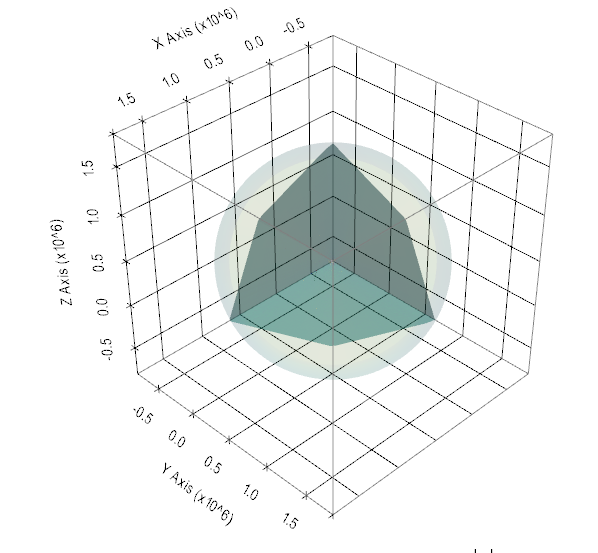
\includegraphics[width=0.9\textwidth]{Figs/mohr_coulomb/MC_octahedral_profile.png}
    \caption{Octahedral profile.}
  \end{subfigure}
  \begin{subfigure}[t]{0.5\textwidth}
    \centering
    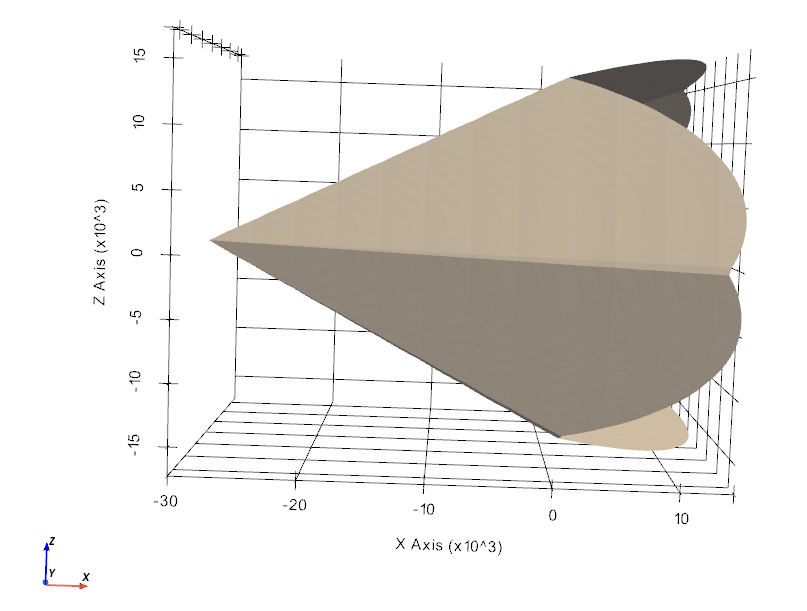
\includegraphics[width=0.9\textwidth]{Figs/mohr_coulomb/MC_rendulic.png}
    \caption{Rendulic profile.}
  \end{subfigure}
  \caption{Profiles of the classical Mohr-Coulomb yield surface.}
  \label{fig:MC}
\end{figure}


\subsection{Sheng et al. yield surface}
The yield function of the Mohr-Coulomb yield surface can be expressed in $p$--$q$ space as
\Beq \label{eq:Sheng}
  f(\Bsig) = q - M p - \tilde{c} \,.
\Eeq
Comparison with \eqref{eq:MC_invariant},
\Beq 
  f(\Bsig) = R(\theta)\,q - p~\sin\phi - c\cos\phi  
\Eeq
indicates that
\Beq 
  M(\theta) = \frac{\sin\phi}{R(\theta)} \quad \Tand \quad \tilde{c}(\theta) = \frac{c\cos\phi}{R(\theta)}
\Eeq
for the classical Mohr-Coulomb model. 
\begin{SummaryBox}[label=box:MC_sheng]{Sheng et al. Mohr-Coulomb yield function}
Sheng et al.~\cite{Sheng2000} suggest a modified model designed for CAMClay type models, which when applied
to the Mohr-Coulomb yield function takes the form
\Beq \label{eq:Sheng_mod}
  f(\Bsig) = q - \tilde{M} p - \tilde{c} \,.
\Eeq
where
\Beq
  \tilde{M}(\theta) = M(\theta=\pi/3) \left(\frac{2\alpha^4}{1 + \alpha^4 + (1 - \alpha^4)\cos3\theta}\right)^{1/4},
  \quad \Tand\quad
  \alpha = \frac{3 - \sin\phi}{3  + \sin\phi} \,.
\Eeq
\end{SummaryBox}
Note that from \eqref{eq:R_theta},
\Beq
  R(\pi/3) = \frac{3 + \sin\phi}{6} \quad \implies \quad
  M(\pi/3) = \frac{6\sin\phi}{3 + \sin\phi}\,.
\Eeq
Plots of the modified yield surface surface in the octahedral and front view are shown in Figure~\ref{fig:MC_Sheng}.
This yield surface is not convex and should be avoided in computations.
\begin{figure}[htbp!]
  \begin{subfigure}[t]{0.5\textwidth}
    \centering
    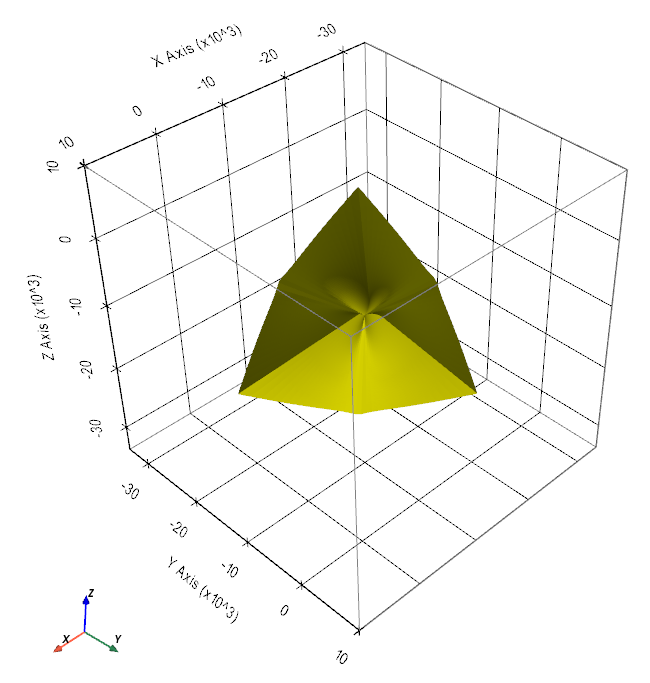
\includegraphics[width=0.7\textwidth]{Figs/mohr_coulomb/MC_sheng_octahedral.png}
  \end{subfigure}
  \begin{subfigure}[t]{0.5\textwidth}
    \centering
    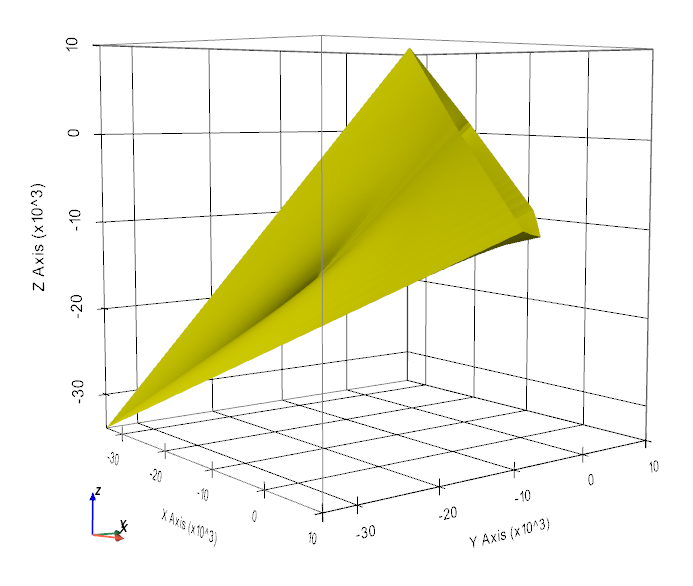
\includegraphics[width=0.7\textwidth]{Figs/mohr_coulomb/MC_sheng_3D.png}
  \end{subfigure}
  \caption{Profiles of the modified Mohr-Coulomb yield surface.}
  \label{fig:MC_Sheng}
\end{figure}
\begin{NoteBox}
Note that the angle $\theta_s$ in \cite{Sheng2000} is defined as
\Beq
  \sin 3\theta_s = -\frac{27}{2} \frac{J_3}{q^3} = -\cos 3\theta ~,~~ \theta_s = \theta - \tfrac{\pi}{6} \,.
\Eeq
For that definition, triaxial compression occurs at $\theta_s = \pi/6$ whereas with our
definition it occurs at $\theta = \pi/3$.
\end{NoteBox}
A variant of the model in \eqref{eq:Sheng_mod} is implemented in \Vaango:
\Beq
  f = \frac{q}{M} - \frac{2c}{M} - p ~,~~
  M = \frac{M_0 \alpha}{\left[\Half \left[1 + \alpha^4 - (1 - \alpha^4) \sin(3\theta_s)\right]\right]^{1/4}} ~,~~
  M_0 = \frac{6\sin\phi}{3 - \sin\phi} \,.
\Eeq
This model is visualized in Figure~\ref{fig:MC_Sheng_imp} and is not convex.
\begin{figure}[htbp!]
  \begin{subfigure}[t]{0.5\textwidth}
    \centering
    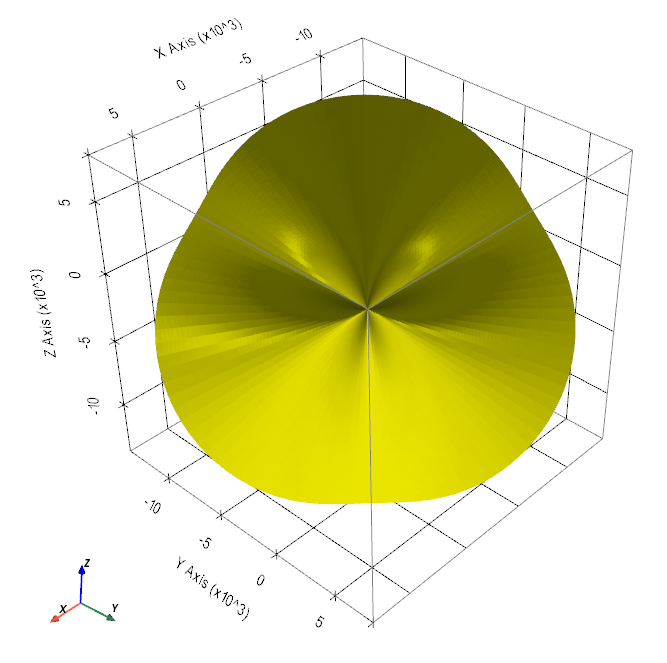
\includegraphics[width=0.7\textwidth]{Figs/mohr_coulomb/MC_sheng_octahedral_imp.png}
  \end{subfigure}
  \begin{subfigure}[t]{0.5\textwidth}
    \centering
    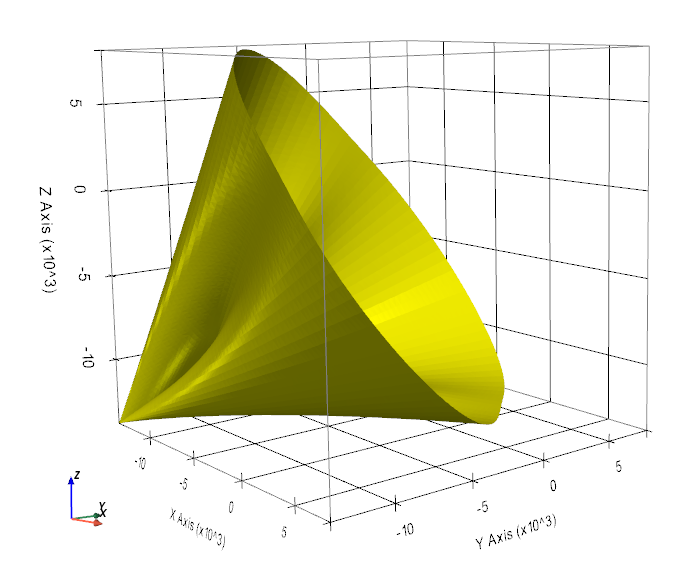
\includegraphics[width=0.7\textwidth]{Figs/mohr_coulomb/MC_sheng_3D_imp.png}
  \end{subfigure}
  \caption{Profiles of the modified Mohr-Coulomb yield surface as implemented in \Vaango.}
  \label{fig:MC_Sheng_imp}
\end{figure}

\section{Variable cohesive strength}
A time varying cohesive strength model can be activated if necessary.  Under certain
circumstances, the cohesive strength is assumed to depend on the effective strain
$\Veps_\Teff$ (see definition in \eqref{eq:eff_strain}) and an effective strain-rate
$\dot{\Veps}_\Teff$.  The strain is computed
from the unrotated rate-of-deformation $\BdT$ using
\Beq
  \BVeps(t_{n+1}) = \BVeps(t_n)  + \BdT \Delta t \quad \text{where} \quad
  \Delta t = t_{n+1} - t_n \,.
\Eeq
The effective strain is then computed using
\Beq
  \Veps_\Teff = \sqrt{
      \tfrac{2}{3}\left[\Third\left[(\Veps_{11} - \Veps_{22})^2 + (\Veps_{22} - \Veps_{33})^2 + (\Veps_{33} - \Veps_{11})^2\right] + 2(\Veps_{12}^2 + \Veps_{23}^2 + \Veps_{13}^2)\right]} \,.
\Eeq
An effective strain-rate, $\dot{\Veps}_\Teff$, is also computed from
\Beq
  \dot{\Veps}_\Teff = \sqrt{
      \tfrac{2}{3}\left[\Third\left[(d_{11} - d_{22})^2 + (d_{22} - d_{33})^2 + (d_{33} - d_{11})^2\right] + 2(d_{12}^2 + d_{23}^2 + d_{13}^2)\right]} \,.
\Eeq

For situations during which a rate-dependent undrained shear transition is important, the
cohesion model takes the form
\Beq
  c(t) = \begin{cases}
            S_t a_1 W^{-b_1} & \quad \text{for}~ \dot{\Veps}_\Teff \le \dot{\Veps}_\Tref \\
            S_t a_1 W^{-b_1} \left(\cfrac{\dot{\Veps}_\Teff}{\dot{\Veps}_\Tref}\right)^\beta & 
               \quad \text{for}~ \dot{\Veps}_\Teff > \dot{\Veps}_\Tref 
         \end{cases}
\Eeq
where $S_t$ is a softening parameter, $a_1, b_1$ are water influence parameters, 
$\dot{\Veps}_\Tref$ is a reference strain-rate, and $\beta$ is a strain-rate parameter.

If the cohesion varies linearly with depth, the model that can be used to compute
depth-dependent values has the form
\Beq
  c(t) = c + A (\Bx_p\cdot\Bn_d  - y_\Tref)
\Eeq
where $A$ is a slope parameter and $y_\Tref$ is a reference depth value. The particle
position is $\Bx_p$ and $\Bn_d$ is the depth direction (aligned with the axes of the computational
domain).

If softening is activated, the cohesive strength is modified if the condition
\Beq
  \Veps_\Teff > \frac{c}{G}
\Eeq
where $c$ is the cohesive strength and $G$ is the shear modulus.  The softening model
has the form
\Beq
  c(t) = c \left[ \frac{1}{S_t} + \left(1 - \frac{1}{S_t}\right) 2.71^{\Veps_\Teff/\Veps_{95}}\right]
\Eeq
where $S_t$ is the softening parameter used earlier and $\Veps_{95}$ is a reference effective strain.

Finally, if a water retention model is used to modify the cohesive strength, a suction value
$\psi_m$ is computed and the cohesion is computed as
\Beq
  c(t) = c + \psi_m \tan\phi_b
\Eeq
where $\phi_b$ is a water retention parameter.  The suction is computed using the van Genuchten
model:
\Beq
 \theta(\psi) = \theta_r + \frac{\theta_s - \theta_r}{\left[ 1+(\alpha |\psi_m|)^n \right]^{1-1/n}}
\Eeq
where $\theta(\psi)$ is the water retention curve, $|\psi_m|$ is the suction pressure,
$\theta_s$ is the saturated water content, $\theta_r$ is the residual water content,
$\alpha > 0$ is a parameter related to the inverse of the air entry suction, and
$n > 1$ is a measure of the pore-size distribution.

\section{Flow rule}
A non-associated flow rule is assumed such that the plastic strain-rate $\BdT_p$ is given by
\Beq
  \BdT_p = \dot{\lambda} \Partial{g}{\Bsig}
\Eeq
where
\Beq
  g(\Bsig) = R(\theta)\,q - p~\sin\psi - c\cos\psi  
\Eeq
and $\psi$ is the dilation angle.  Typically $\psi$ is taken to be equal to $\phi$, the friction
angle.

The normal to the plastic potential surface is given by
\Beq
  \BnT = \Partial{g}{\Bsig}  = \Deriv{R}{\theta}\Partial{\theta}{\Bsig} \,q 
                              + R(\theta)\, \Partial{q}{\Bsig} 
                              - \Partial{p}{\Bsig}~\sin\psi \,.
\Eeq
where
\Beq
  \Bal
  \Deriv{R}{\theta} & = \tfrac{1}{\sqrt{3}}~\cos\left(\theta+\cfrac{\pi}{3}\right) +
                      \tfrac{1}{3}\sin\psi~\sin\left(\theta+\cfrac{\pi}{3}\right)  \\
  \Partial{\theta}{\Bsig} & = 
     -\frac{1}{\sin 3\theta}\left[\frac{9}{2 q^3} \Partial{J_3}{\Bsig} - \frac{r^3}{q^4} \Partial{q}{\Bsig}\right]
   = -\frac{1}{\sin 3\theta}\left[\frac{9}{2 q^3} \left(\Bs \cdot \Bs - \tfrac{2}{3} J_2 \BI\right) - \frac{r^3}{q^4} \Partial{q}{\Bsig} \right] \\
  \Partial{q}{\Bsig} & = \frac{\sqrt{3}}{2\sqrt{J_2}} \Partial{J_2}{\Bsig}
                     = \frac{\sqrt{3}}{2\sqrt{J_2}} \Bs  \\
  \Partial{p}{\Bsig} & = \tfrac{1}{3} \Partial{I_1}{\Bsig} = \tfrac{1}{3} \BI \,.
  \Eal
\Eeq

\section{Nonlocal shear correction}
The Mohr-Coulomb model contains a nonlocal correction feature that
uses neighbor information to regularize solutions.  Neighboring particles that
contribute to the nonlocal effect are identified using a nonlocal length ($\ell_n$).
Let there be $N_q$ such particles in the neighborhood of particle $p$.

The nonlocal effective strain ($\Veps_\Teff^n$) and effective strain rate ($\dot{\Veps}_\Teff^n$)
are computed as
\Beq
  \Veps_\Teff^n = (1 - n) \Veps_\Teff + n \left(\cfrac{\sum_{q=1}^{N_q} V_w^q \Veps_\Teff}{\sum_{q=1}^{N_q} V_w^q}\right)
  \quad \Tand \quad
  \dot{\Veps}_\Teff^n = (1 - n) \dot{\Veps}_\Teff + n \left(\cfrac{\sum_{q=1}^{N_q} V_w^q \dot{\Veps}_\Teff}{\sum_{q=1}^{N_q} V_w^q}\right)
\Eeq
where $n$ is a nonlocal parameter, $\Veps_\Teff, \dot{\Veps}_\Teff$ are the local effective strain
and strain-rate, respectively, and $V_w^q$ is a weighted volume of neighboring particle $q$ whose
local volume is $V_q$.  The expression for $V_w^q$ is
\Beq
  V_w^q = w_{pq} V_q \quad \text{where} \quad 
   w_{pq} = \frac{\ell}{\ell_n}\exp\left(-\frac{\ell^2}{\ell_n^2}\right) ~,~~
   \ell = \Norm{\Bx_q - \Bx_p}{} \,.
\Eeq
If a regularization flag is activated, and $\Veps_\Teff^n > c/G$, where $c$ is the cohesion and $G$ is
the shear modulus, a time-scale is included in the computation:
\Beq
  \Veps_\Teff^n \leftarrow  \Veps_\Teff^n \frac{t_{\text{FE}}}{t_{\text{shear}}} ~,~~
  \dot{\Veps}_\Teff^n \leftarrow  \dot{\Veps}_\Teff^n \frac{t_{\text{FE}}}{t_{\text{shear}}}  \,.
\Eeq
where $t_{\text{FE}}$ and $t_{\text{shear}}$ are regularization time scales.  The nonlocal 
effective strain is typically not used directly in the model except for modifying the cohesion
and the elastic moduli.
 
However, after the stress has been updated, a nonlocal correction can be applied using a similar
approach:
\Beq
  \Bsig^n = (1 - n) \Bsig + n \left(\cfrac{\sum_{q=1}^{N_q} V_w^q \Bsig}{\sum_{q=1}^{N_q} V_w^q}\right)
\Eeq
where $\Bsig_n$ is the nonlocal stress. 

\section{Explicit stress integration}
An additive decomposition of the unrotated rate-of-deformation into elastic and plastic parts is assumed:
\Beq
  \BdT = \BdT_e + \BdT_p
\Eeq
Elastic and plastic strains are defined using
\Beq
  \BVeps = \int_0^t \BdT(\tau) d\tau  = \BVeps_e + \BVeps_p \quad \implies \quad 
  \BVeps_e = \int_0^t \BdT_e(\tau) d\tau ~,~~ \BVeps_p = \int_0^t \BdT_p(\tau) d\tau \,.
\Eeq
The strain increment during a timestep, $\Delta t = t_{n+1} - t_n$, is computed as
\Beq
  \Delta\BVeps = \BdT \Delta t \,.
\Eeq
The stress update begins with a check whether the stress state at the beginning of the
time step is on the yield surface.  This is necessary because the modification of the cohesion
and the elastic moduli may have affected the shape of the yield surface.
Special checks are used to determine if the strain increment leads to unloading.  Details
are omitted for brevity.

An elastic trial stress state is computed
\Beq
  \Bsig^\Trial = \Bsig_n + \SfC_n : \Delta\BVeps
\Eeq
where $\SfC$ tangent elastic modulus tensor.

If the trial stress is in the plastic region, the intersection of the stress increment
vector $\Delta \Bsig = \Bsig^\Trial - \Bsig_n$ with the yield surface is 
computed using bisection.  The strain increment corresponding to this reduced stress
increment is the increment in elastic strain and the stress on the yield surface is
the stress at the end of the elastic strain increment.

The remainder of the strain increment is purely plastic.  The trial stress now has to be
projected back to the yield surface along the projection vector $\BP$~\cite{Brannon2000a}, given by
\Beq  
  \BP = -\SfC : \Partial{g}{\Bsig} \,.
\Eeq  
The intersection of the projection vector with the yield surface is found via bisection.
The updated stress is the intersection point on the yield surface.

Several Runge-Kutta schemes are implemented in the \Vaango code to break-up large
The intersection of the projection vector with the yield surface is found via bisection.
strain increments into smaller steps.  However, the two-step modified Euler scheme is accurate
enough for our purposes.

This procedure is repeated for each timestep.
